\section{The TOV equation}

We will model a star as being made up of a \emph{perfect fulid}, with energy density $\rho$ and pressure $p$.
The relationship between the pressure and energy density of a substance is called the \emph{equation of state}, or EOS, and has the form
\begin{equation}
    \label{EOS}
    f(p, \rho, \{\xi_i\}) = 0,
\end{equation}
where $\{\xi_i\}$ are possible other thermodynamic variables.
We will be working at zero temperature, in which case there are no other free thermodynamic variables.
This allows us to, at least locally, express the pressure as a function of the energy density, $p = p(\rho)$.
The stress-energy tensor of a perfect fluid is\todo{Forklar}
%
\begin{equation}
    T_{\mu \nu} = (\rho + p) u_\mu u_\nu - p g_{\mu \nu},
\end{equation} 
where $u_\mu$ is the 4-velocity of the fluid.
In the rest frame of the fluid, we may write 
\begin{equation}
    u_\mu = \left(u_0, 0, 0, 0\right).
\end{equation}
This, together with the normalization condition of 4-velocities, $u_\mu u^\mu = 1$, allows us to calculate that
%
\begin{equation}
    u_\mu u^\mu = g^{\mu \nu} u_\mu u_\nu = g^{00} (u_0)^2 = 1.
\end{equation}
%
Using \autoref{spherically symmetric metric}, we see that
\begin{equation}
    u_0 = e^{\alpha(r)}.
\end{equation}
%
This gives us the stress-energy tensor of the perfect fluid in its rest frame,
%
\begin{equation}
    T_{\mu \nu} 
    =
    \left(
        \begin{matrix}
            \rho{\left(r \right)} e^{2 \alpha{\left(r \right)}} & 0 & 0 & 0\\0 & 
            p{\left(r \right)} e^{2 \beta{\left(r \right)}} & 0 & 0\\
            0 & 0 & p{\left(r \right)} r^{2} & 0\\
            0 & 0 & 0 & p{\left(r \right)} r^{2} \sin^{2}{\left(\theta \right)}
        \end{matrix}
    \right).
\end{equation}
%
We will use the $tt$ and $rr$ components of the Einstein field equations, which are
%
\begin{align}
    \label{tt equation}
    8 \pi G r^{2} \rho{\left(r \right)} e^{2 \beta{\left(r \right)}} 
    & =   2 r \frac{d}{d r} \beta{\left(r \right)} + e^{2 \beta{\left(r \right)}} - 1 \\
    \label{rr equation}
    8 \pi G r^{2} p{\left(r \right)} e^{2 \beta{\left(r \right)}} 
    & = 2 r \frac{d}{d r} \alpha{\left(r \right)} - e^{2 \beta{\left(r \right)}} + 1.
\end{align}
%
In analogy with the Schwartzhild metmric, we define the function $m(r)$ by
\begin{equation}
    e^{2 \beta(r)} = \left(1 - \frac{2 G m(r)}{r} \right)^{-1}. 
\end{equation}
Substituting this into \autoref{tt equation} yields 
\begin{equation}
    \diff{m(r)}{r} = 4 \pi r^2 \, \rho(r).
\end{equation}
The solution is simply
\begin{equation}
    \label{mass relation}
    m(r) = 4 \pi \int_0^r \dd r' \, {r'}^2 \rho(r').
\end{equation}
We see that $m(r)$ is the matter content contained within a radius $r$.
If $\rho = 0$ for $r > R$ and $m(r>R) = M$, then the metric on a constant-time surface, i.e. $\dd t = 0$, is
%
\begin{equation}
    \dd s^2
    = 
    \left( 1 - \frac{2 G M}{r^2} \right)^{-1} \dd r^2 
    + r^2 (\dd \theta^2 + \sin^2 \theta \, \dd\varphi^2),
\end{equation} 
%
which is the same as the for the Schwartzhild solution.

Using the Bianchi identity, \autoref{Einstein tensor bianchi identity}, together with EInstein's equation, we find that
%
\begin{equation}
    \nabla^\mu G_{\mu \nu} = \nabla^\mu T_{\mu \nu} = 0.
\end{equation}
%
The $r$-component of this equation is
%
\begin{equation}
    \nabla_\mu T^{\mu r} 
    =
    \partial_r T^{rr} 
    + \Gamma^\mu_{\mu \nu} T^{\nu r} 
    + \Gamma^r_{\mu \nu} T^{\mu \nu},
\end{equation}
%
where we have used the particular form of $T_{\mu \nu}$ and the Christoffel symbols to eliminate vanishing terms.
We calculate
%
\begin{align*}
    \nabla_\mu T^{\mu r} 
    & = 
    \partial_r \left(p e^{-2\beta}\right)
    + (2 \Gamma^r_{rr} + \Gamma^t_{tr}) T^{rr} 
    + \Gamma^r_{tt}T^{tt} \\ 
    &=   e^{-2\beta} \left( \partial_r p + p \partial_r \alpha + \rho \partial_r \alpha \right) = 0.
\end{align*} 
%
This allows us to relate $\alpha$ to $p$ and $\rho$, via
\begin{equation}
    \partial_r \alpha = - \frac{\partial_r p}{p + \rho}
\end{equation}
When we substitute this, together with the definition of $m(r)$, into \autoref{rr equation}, we obtain
\begin{equation}
    \label{TOV}
    \diff{p}{r}
    =
    -
    \frac{
        G \left(4 \pi r^{3} p + m \right) \left(\rho + p \right)
        }
        {r \left(r- 2 G m\right)},
\end{equation}
the Tolman-Oppenheimer-Volkoff (TOV) equation.

To summarize, we have three functions describeing the star, $\rho$, $p$, and $m$, as well as thre equations, \autoref{EOS}, \autoref{mass relation} and \autoref{TOV}.
Together with inital conditions, such as $p(0) = p_0$, this is enough to determin the unknown funcions.
For completness, the equations are
\todo{Bytt notasjon - $\rho \rightarrow u$.}
\begin{align*} 
    0 & = f(P, u) , \\
    \diff{m}{r} & = 4 \pi r^2 u(r), \\
    \diff{p}{r} & =
    -
    \frac{G \left(4 \pi r^{3} p + m \right) \left(u + p \right)}{r \left(r- 2 G m\right)}.
\end{align*}


\subsection*{Incompressible fluid}

The simples model for a fluid is an incompressible fluid, where the energy density is independent of the pressure.
In this case, the energy density of the star will be constant for a radius $r < R$, before it drops to zero,
%
\begin{equation}
    \rho(r) = \rho_0 \, \theta (R - r),
\end{equation}
%
where $\rho_0$ is a constant and $\theta(x)$ the Heaviside step funciton.
The mass of the star, for $r < R$, is
%
\begin{equation}
    m(r) = \frac{4 \pi }{3} r^3 \rho_0.
\end{equation}
%
Inserting this into \autoref{TOV}, this yields
%
\begin{equation} 
    \diff{p'}{r'} = - \frac{M r (1 + p')(1 + 3 p')}{(1 - 2 M r')}.
\end{equation}
%
Here, we have made the definitions
%
\begin{equation}
    p' \rho_0 = p, \quad R r' = r, \quad
    M = G \frac{4 \pi}{3} R^3 \rho_0.
\end{equation}
%
This is a separable ODE, which means that each varaibel may integrated separly:
%
\begin{align}
    \int \frac{\dd p'}{(1 + p')(1 + 3p')} 
    = \frac{1}{2} \ln \frac{p' + \frac{1}{3}}{p' + 1} + \const , \\
    \int \frac{\dd r' \, M r'}{(2 M r'^2 - 1)} = \frac{1}{4}\ln\left(2 r'^2 - 1 \right) + \const
\end{align}
%
Combining these, together with the boundary condition $p'(r' = 1) = 0$, we get
%
\begin{equation}
    p'(r') = - \frac{\sqrt{1 - 2M} - \sqrt{1 -2Mr'^2}}{3 \sqrt{1 - 2M} - \sqrt{1 - 2M r'^2} }.
\end{equation}
%
We see that, if the mass exceeds the critical value
%
\begin{equation}
    M_0 = \frac{4}{9},
\end{equation}
then the pressure will diverge towards the centrum.
General relativity does not allow for static solution with energy densities greater than this~\autocite{carrollSpacetimeGeometryIntroduction2019}.
The pressure as a function of radius of the incompressible fluid is illustrated in \autoref{fig: pressure incompressible fluid}.
Here, each line corresponds to a value for $M$ within the indicated range, close to the critical value $M_0$.
Notice how this will scale the $y$-axis as this corresponds to different values for $\rho_0$.

\begin{figure}
    \centering
    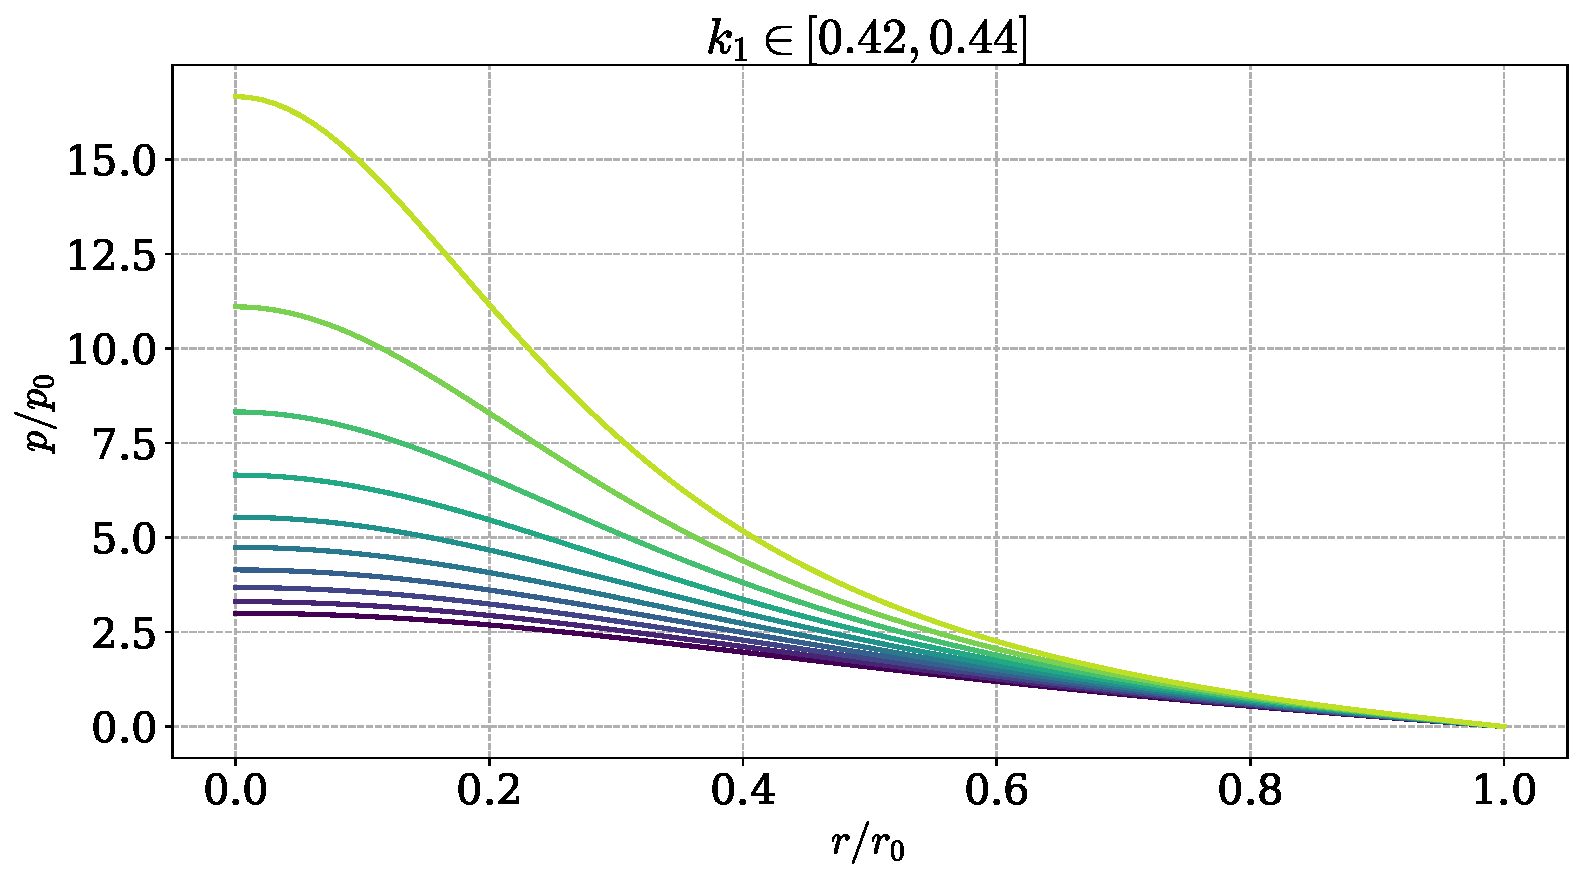
\includegraphics[width=0.8\textwidth]{figurer/scripts/incompressible.pdf}
    \caption{The pressure of a star made up of a incompressible fluid, as a funciton of its radius. The different lines corresponds to different total masses, and thus also different energy densities $\rho_0$. Notice how this will change the $y$-axis for each line.}
    \label{fig: pressure incompressible fluid}
\end{figure}

\subsection*{Free fermi gas}

A non-interacting free Fermi gas is goverened by the Lagrangian
\todo{Skrive om thermal field theory}
%
\begin{equation}
    \Ell = \bar \psi (i \slashed \partial - m) \psi.
\end{equation}
%
This gas has the free energy density, after droping a infinite constant, 
%
\begin{equation}
    \Eff = \frac{2}{\beta}\int \frac{\dd^3 p}{(2 \pi)^3} \left[
        \ln(1 + e^{-\beta(\omega - \mu)})
        + 
        \ln(1 + e^{-\beta(\omega + \mu)})
    \right],
\end{equation}
%
where $\omega = \sqrt{p^2 + m^2}$.
%
\begin{equation}
    \int_0^\infty \ln\left[1 + e^{-\beta(\omega \pm m)}\right]
    = 
    \frac{1}{3} p^3\ln\left[1 + e^{-\beta(\omega \pm m)}\right] \bigg |_0^\infty
    + \frac{1}{3} \int_0^\infty \dd p \, \frac{ \beta p^4}{\omega}n_f(\omega \pm \mu),
\end{equation}
%
where
%
\begin{equation}
    n_f(\omega) = \frac{1}{e^{\beta \omega}+1}.
\end{equation}
%
Thermodynamcs:
%
\begin{equation}
    P = - \Eff, \quad n = - \diffp{\Eff}{\mu}, \quad u = \Eff + \mu n.
\end{equation}
%

Thus,
%
\begin{equation}
    P = \frac{2}{3}\int \frac{\dd^3 p}{(2 \pi)^3} 
    \frac{p^4}{\omega}
    [n_f(\omega - \mu) + n_f(\omega + \mu)]
\end{equation}
%

%
\begin{equation}
    n = 2 \int \frac{\dd^3 p}{(2 \pi)^3}
    \left[
        n_f(\omega + \mu)
        -
        n_f(\omega - \mu)
    \right]
\end{equation}
%

%
\begin{equation}
    u
    =
    -\frac{1}{\pi^2}
    \int \dd p \,
    p^2
    \left[
        \left(
            \frac{1}{3}
            \frac{p^2}{\omega}
            -
            \mu
        \right)
        n_f(\omega - \mu)
        +
        \left(
            \frac{1}{3}
            \frac{p^2}{\omega}
            +
            \mu
        \right)
        n_f(\omega + \mu)
    \right]
\end{equation}
%

Define $\mu = \sqrt{p_f^2 - m^2}$.
with $\beta \rightarrow \infty$, and $\mu = \sqrt{p_f^2 + m^2}$, we have
%
\begin{align}
    &\int_0^\infty \dd p \, p^2  \sqrt{p^2 + m^2} n(\omega - \mu)
    =
    \int_0^{p_f} \dd p \, p^2 \sqrt{p^2 + m^2}\\
    & = \frac{1}{3} p^3 \sqrt{p^2 + m^2 }\bigg|_0^{p_f} 
    - \frac{1}{3}\int_0^{p_f} \dd p \, \frac{p^4}{\sqrt{p^2 + m^2}}.
    =
    -
    \int_0^{p_f}
    \dd p \, p^2
    \left(
        \frac{1}{3}
        \frac{p^2}{\omega}
        - \mu
    \right).
\end{align}
%
Thus,
%
\begin{align}
    u &= \frac{1}{\pi^2} \int_0^{p_f} \dd p \,
    p^2 \sqrt{p^2 + m^2}
    = \frac{m^4}{\pi^2} \int_0^{x_f} \dd x \, x^2 \sqrt{x^2 + 1}, \\
    P & = \frac{1}{3 \pi^2} \dd p \, \int_0^{p_f}\frac{p^4}{\sqrt{p^2 + m^2}} 
    = \frac{m^4}{3 \pi^2} \int_0^{x_f} \frac{\dd x \, x^4}{\sqrt{x^2 + 1}}.
\end{align}
%
Using 
%
\begin{align}
    \int_0^a \dd x \, x^2 \sqrt{x^2 + 1} 
    & = \frac{1}{8} 
    \left[a \sqrt{a^2 + 1}(2 a^2 + 1) - \ln\left(\sqrt{a^2 + 1} + a\right)\right], \\
    \int_0^a \dd x \, \frac{x^4}{\sqrt{x^2 + 1} }
    & = \frac{1}{8} 
    \left[a \sqrt{a^2 + 1}(2 a^2 - 3) + 3\ln\left(\sqrt{a^2 + 1} + a\right)\right].
\end{align}
%
We get 
%
\begin{align}
    u &= \frac{m^4}{8 \pi^2} 
    \left[\mu x_f (2x_f^2 + 1) - \ln\left(\mu + x_f\right)\right], \\
    P &= \frac{m^4}{24 \pi^2} 
    \left[\mu x_f (2x_f^2 -3) + 3\ln\left(\mu + x_f\right)\right].
\end{align}
%
eqs
%
\begin{align}
    \diff{p}{r} = - \frac{(4 \pi r^3 P + m)(u + P)}{r(r - 2 m)} \\
    \diffp{m}{r} = 4 \pi r^2 u
\end{align}